% CS70--Spring 2024 --- Discussion 2B Solutions
\documentclass[11pt]{article}
\usepackage{amsmath,textcomp,amssymb,geometry,graphicx,enumerate}
\usepackage{xeCJK}

\def\Name{JayZhao}  % Your name
\def\SID{0}  % Your student ID number-
\def\Homework{2B} % Number of Homework
\def\Session{Spring 2024}

\title{CS70--Spring 2024 --- Discussion \Homework \ Solutions}
\author{\Name, SID \SID}
\markboth{CS70--\Session\  Discussion \Homework\ \Name}{CS70--\Session\ Discussion \Homework\ \Name}
\pagestyle{myheadings}
\date{\today}

\newenvironment{qparts}{\begin{enumerate}[{(}a{)}]}{\end{enumerate}}

\def\endproofmark{$\Box$}
\newenvironment{proof}{\par{\bf 证明}:}{\endproofmark\smallskip}

\textheight=9in
\textwidth=6.5in
\topmargin=-.75in
\oddsidemargin=0.25in
\evensidemargin=0.25in

\begin{document}
\maketitle

% 1. 简答题

\section*{1. 简答题}
\begin{qparts}
\item 一个连通的平面简单图比其顶点多5条边。它有多少个面?
\begin{proof}
设图的顶点数为 $v$,边数为 $e$。题目说“比其顶点多5条边”,即 $e = v + 5$。

平面连通图满足欧拉公式:
\[
    v - e + f = 2
\]
其中 $f$ 表示面的数量。
将 $e = v + 5$ 代入欧拉公式:
\[
    v - (v+5) + f = 2 \\
    v - v - 5 + f = 2 \\
    -5 + f = 2 \\
    f = 7
\]
所以,这个图有 $7$ 个面。

\textbf{补充说明:} 欧拉公式是平面连通图的基本性质,适用于所有无自环、无重边的平面连通图。
\end{proof}

\item 从一个3维超立方体中需要移除多少条边才能得到一棵树?
\begin{proof}
首先,3维超立方体的顶点数为 $2^3 = 8$。每个顶点与3个其他顶点相连(因为每个比特位都可以变化一次),所以每个顶点度为3。

总边数为:
\[
    \text{总度数} = 8 \times 3 = 24 \\
    \text{总边数} = \frac{24}{2} = 12
\]
(每条边被两个顶点计数,所以要除以2)

一棵树有 $n$ 个顶点时,边数为 $n-1$。所以8个顶点的树有 $8-1=7$ 条边。

因此,需要移除 $12-7=5$ 条边,才能把3维超立方体变成一棵树。

\textbf{补充说明:} 超立方体本身是一个连通且有环的图,去掉足够的边使其无环且连通,就是生成树。
\end{proof}

\item 欧拉公式 $v-e+f=2$ 要求平面图是连通的。对于有 $k$ 个连通分量的平面图,其类似的公式是什么?
\begin{proof}
对于有 $k$ 个连通分量的平面图,每个连通分量单独满足 $v_i - e_i + f_i = 2$。但所有分量的面数之和要减去重复计算的外部面(所有分量共享一个外部面)。

设总顶点数为 $v$,总边数为 $e$,总面数为 $f$,则:
\[
    \sum_{i=1}^k (v_i - e_i + f_i) = 2k
\]
但所有分量的外部面实际上是同一个,所以总面数 $f = \sum f_i - (k-1)$。

整理得:
\[
    v - e + f = k + 1
\]
\textbf{例子:} 两个分离的三角形($k=2$),总顶点6,总边6,总面3(每个三角形2个面,合并外部面),代入公式 $6-6+3=3=2+1$。
\end{proof}
\end{qparts}

% 2. 总是、有时或从不

\section*{2. 总是、有时或从不}
\begin{qparts}
\item G 可以用4种颜色进行顶点着色。
\begin{proof}
\textbf{有时。} 4-可着色并不意味着一定平面,也不意味着一定非平面。

\textbf{例子1(平面图)}:$K_4$(4个顶点的完全图)是平面图,且需要4种颜色。

\textbf{例子2(非平面图)}:$K_{3,4}$(3-4二分图)不是平面图,但也可以4-可着色。

\textbf{结论:} 仅知道4-可着色,无法判断G是否平面。
\end{proof}

\item G 需要7种颜色才能进行顶点着色。
\begin{proof}
\textbf{总是不平面的。}

根据四色定理,所有平面图都最多4-可着色。如果一个图需要7种颜色,说明它的色数大于4,因此一定不是平面图。

\textbf{补充说明:} 例如完全图$K_7$需要7种颜色,但$K_7$不是平面图。
\end{proof}

\item $e \le 3v-6$,其中 $e$ 是 G 的边数,$v$ 是 G 的顶点数。
\begin{proof}
\textbf{有时。}

$e \le 3v-6$ 是平面简单图的必要条件,但不是充分条件。

\textbf{例子1(平面图)}:$K_4$,$v=4, e=6, 3v-6=6$,满足条件且是平面图。

\textbf{例子2(非平面图)}:$K_{3,3}$,$v=6, e=9, 3v-6=12$,满足条件但不是平面图。

\textbf{结论:} 满足 $e \le 3v-6$ 不能保证图一定平面。
\end{proof}

\item G 是连通的,并且 G 中的每个顶点的度数最多为2。
\begin{proof}
\textbf{总是平面的。}

这样的图只能是路径或环(连通且每点度数最多2)。

\textbf{例子1:} 路径 $1-2-3-4$。

\textbf{例子2:} 环 $1-2-3-4-1$。

这些图都可以画在平面上且无交叉。
\end{proof}

\item G 中的每个顶点的度数最多为2。
\begin{proof}
\textbf{总是平面的。}

这样的图是若干个路径和环的并(不要求连通)。每个分量都可以单独画在平面上且无交叉。

\textbf{例子:} 两个不相交的环,或一个环加一条路径。
\end{proof}
\end{qparts}

% 3. 图着色

\section*{3. 图着色}
\begin{proof}
设图的最大度数为 $k$,我们要证明它一定 $(k+1)$-可着色。

\textbf{思路:} 用归纳法。

\textbf{基础情形}:只有1个顶点时,显然1-可着色。

\textbf{归纳假设}:假设所有$n-1$个顶点的最大度不超过$k$的图都可以用$k+1$种颜色着色。

\textbf{归纳步骤}:对$n$个顶点的图,任选一个顶点$v$,删去$v$后,剩下的图最大度仍不超过$k$,可用$k+1$色着色。将$v$加回,$v$最多有$k$个邻居,最多用掉$k$种颜色,所以总有一种颜色可分配给$v$。

\textbf{结论:} 归纳成立,最大度为$k$的图一定$(k+1)$-可着色。
\end{proof}

% 4. 超立方体

\section*{4. 超立方体}
\begin{qparts}
\item 画出1维、2维、3维超立方体,并标记比特串。

\textbf{1维:}

两个点$0,1$,一条边:

\begin{center}
\begin{tabular}{c}
$0$ --- $1$
\end{tabular}
\end{center}

\textbf{2维:}

四个点$00,01,10,11$,边连接相差一位的点:

\begin{center}
\begin{tabular}{cc}
$00$ --- $01$ \\
$|$ \hspace{1.5cm} $|$ \\
$10$ --- $11$
\end{tabular}
\end{center}

\textbf{3维:}

八个点$000,001,010,011,100,101,110,111$,每条边连接仅一位不同的点。可以画成立方体:

\begin{center}
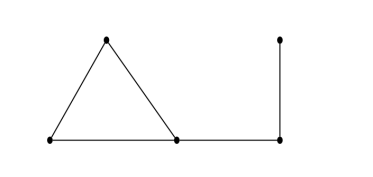
\includegraphics[width=0.3\linewidth]{week2/image-1.png}
\end{center}

\item 证明n维超立方体的边可以用n种颜色着色,使得每个顶点的相邻边颜色都不同。
\begin{proof}
对每一位$i$($1 \leq i \leq n$),将所有第$i$位不同的边染成第$i$种颜色。即,若两个顶点的比特串仅第$i$位不同,则它们之间的边染成第$i$种颜色。

每个顶点有$n$条边,分别对应比特串的每一位变化,因此每条边颜色都不同。

\textbf{例子:} 3维超立方体中,$000$与$001$仅第3位不同,对应第3种颜色。

\textbf{结论:} 这样染色后,每个顶点的相邻边颜色都不同。
\end{proof}

\item 证明n维超立方体是二分图。
\begin{proof}
将所有比特串中1的个数为偶数的点分为一组,奇数的分为另一组。

每条边连接的两个点必然一奇一偶(因为只改变一位,1的个数奇偶性改变)。

\textbf{例子:} $000$(偶)与$001$(奇)相连。

\textbf{结论:} 没有同组内的边,故是二分图。
\end{proof}
\end{qparts}

\end{document}
